\documentclass[a4paper]{article}
\usepackage[14pt]{extsizes}
\usepackage{amssymb}  %  Математические символы
\usepackage{amsmath}  %  Математический пакет
\usepackage{amsthm}  %  Пакет для использования теорем
\usepackage{caption}  %  Пакет для использования подписей
\usepackage{misccorr}  %  Пакет с большинством настроек русских типографических правил - точки после цифр в оглавлении, etc.
\usepackage[noadjust]{cite}
\usepackage{cmap} % Для возможности нормального поиска в тексте и копирования
%  cmap должен быть подключен раньше babel !
\usepackage[utf8]{inputenc}  %  Кодировка исходного файла, который я тут вижу
\usepackage[T2A]{fontenc}  %  Набор символов на выходе, T2A включает в себя кириллицу
\usepackage[german, english, russian]{babel}
\usepackage{graphics}
\usepackage{graphicx}
\usepackage{indentfirst}  %  Либо подключать этот пакет, либо писать каждый раз \indentfirst в начале каждой главы (на Западе не ставят первую красную строку)
\usepackage{verbatim}  %  Окружение для вставки raw-кода
\usepackage{makeidx}
\usepackage{geometry}  %  Настройка геометрии вёрстки -- например, полей
\usepackage{hyperref}
\usepackage{fancyvrb}
\usepackage{color} %% это для отображения цвета в коде
\usepackage{listings} %% собственно, это и есть пакет listings
\usepackage{wrapfig}
\usepackage{setspace}

\DeclareCaptionFont{white}{\color{white}} %% это сделает текст заголовка белым
%% код ниже нарисует серую рамочку вокруг заголовка кода.
\DeclareCaptionFormat{listing}{\colorbox{gray}{\parbox{\textwidth}{#1#2#3}}}
\captionsetup[lstlisting]{format=listing,labelfont=white,textfont=white}
\DeclareGraphicsExtensions{.pdf,.png,.jpg}

\geometry{pdftex, left = 2cm, right = 2cm, top = 2.5cm, bottom = 2.5cm}
\righthyphenmin = 2
\begin{document}
	\begin{titlepage}
		\centering
		\begin{wrapfigure}[7]{l}{0.14\linewidth}
			\vspace{5mm}
			\hspace{-5.8mm}
			
\includegraphics[width=0.93\linewidth]{gerb}
		\end{wrapfigure}
		{\singlespacing \footnotesize \bfseries Министерство науки и высшего образования Российской Федерации\\Федеральное государственное бюджетное образовательное учреждение\\высшего образования\\<<Московский государственный технический университет\\имени Н.~Э.~Баумана\\ (национальный исследовательский университет)>>\\(МГТУ им. Н.~Э.~Баумана)\\}
		
		\textbf {\bf \underline{\hspace{\linewidth}}}
	
		\doublespacing \small \raggedright ФАКУЛЬТЕТ \hspace{25mm} \underline { «Информатика и системы управления»}\\
		КАФЕДРА \hspace{5mm} \underline {«Программное обеспечение ЭВМ и информационные технологии»}\\
		
		\vspace{30mm}
		\begin{center}
		\textbf{Отчёт по лабораторной работе №1}\\
		{\bf	По дисциплине: <<Анализ алгоритмов>>}\\
		{\bf Тема:} \underline {<<Вычисление редакционного расстояния>>}\\
		\end{center}
		\begin{flushleft}
			{\bf Студент}  \underline{Мередова Айджахан}\underline {\hspace{7cm}}
			\newline
			{\bf Группа} \underline{ИУ7-56Б}\underline {\hspace{10cm}}
			\newline
			{\bf Преподаватели} \underline {Волкова Л.Л., Строганов Ю.В.}
		\end{flushleft}

		\vfill
		
		\centering Москва - 2020 г.\\
	\end{titlepage}
	\lstset{ %
		language=Python,                 % выбор языка для подсветки 
		basicstyle=\small\sffamily, % размер и начертание шрифта для подсветки кода
		%numbers=left,               % где поставить нумерацию строк (слева\справа)
		numberstyle=\tiny,           % размер шрифта для номеров строк
		stepnumber=1,                   % размер шага между двумя номерами строк
		numbersep=5pt,                % как далеко отстоят номера строк от подсвечиваемого кода
		backgroundcolor=\color{white}, % цвет фона подсветки - используем \usepackage{color}
		showspaces=false,            % показывать или нет пробелы специальными отступами
		showstringspaces=false,      % показывать или нет пробелы в строках
		showtabs=false,             % показывать или нет табуляцию в строках
		frame=single,              % рисовать рамку вокруг кода
		tabsize=2,                 % размер табуляции по умолчанию равен 2 пробелам
		captionpos=t,              % позиция заголовка вверху [t] или внизу [b] 
		breaklines=true,           % автоматически переносить строки (да\нет)
		breakatwhitespace=false, % переносить строки только если есть пробел
		escapeinside={\%*}{*)}   % если нужно добавить комментарии в коде
	}

	\section*{Введение}Расстояние Левенштейна (также редакционное расстояние или дистанция редактирования) между двумя строками в теории информации и компьютерной лингвистике — это минимальное количество операций вставки одного символа, удаления одного символа и замены одного символа на другой, необходимых для превращения одной строки в другую.
	Впервые задачу упомянул в 1965 году советский математик Владимир Иосифович Левенштейн при изучении последовательностей. Впоследствии более общую задачу для произвольного алфавита связали с его именем. Большой вклад в изучение вопроса внёс Дэн Гасфилд.
	\section{Аналитическая часть}
	\subsection{Постановка задачи}
	{\bf Цель данной лабораторной работы:} разработать и сравнить алгоритмы поиска расстояний Левенштейнаи Демерау-Левенштейна с использованием метода динамического динамического программирования.
	\newline
	В данной работе требуется:
	\begin{enumerate}
		\item описать алгоритмы поиска Левенштейна и Демерау - Левенштейна лдля нахождения редакционного расстояния между строками;
		\item реализовать данные алгоритмы на одном из языков программирования;
		\item провести сравнительный анализ алгоритмов по затраченному времени и памяти;
		\item привести пример работы всез указанных алгоритмов;
	\end{enumerate}
	\subsection{Описание расстояния}
	\subsubsection{Расстояние Левенштейна} Для поиска расстояния Левенштейна, чаще всего используют алгоритм, в котором необходимо заполнить матрицу D, размером n+1 на m+1, где n, m - длины сравниваемых строк A и B, по следующим правилам:
	\begin{itemize}
		\item $D_{0,0} = 0$;
		\item $D_{i,j} = $ минимальное из:
		\begin{itemize}
			\item $D_{i-1, j-1+0}$(мисволы одиноковые), либо $D{i-1, j-1} + $ Creplace(замена символа);
			\item $D_{i, j-1}$ + Cdelete(удаление символа);
			\item $D_{i-1, j}$ + Cinsert(Вставка символа);
		\end{itemize}
	\end{itemize}
	где Creplace, Cdelete, Cinsert - цена или вес замены, удаления и вставки символа. При этом $D_{n-1, m-1}$ - содержит значение расстояния Левенштейна.
	
	Пусть S1 и S2 - две строки(длиной n и m соответственно) над некоторым алфавитом, тогда редакционное расстояние D(S1,S2) можно подсчитать по следующей рекуррентной формуле:
	\begin{equation} 
		D(S_1[i]S_2[j]) = min 
			\begin{cases}
				D(S_1[1..i], S_2[1..j-1]) + 1;\\
				D(S_1[1..i-1], S_2[1..j]) + 1;\\
				D(S_1[1..i-1], S_2[1..j-1]) + \begin{cases}
					0, \text {если}  S_1[i] = S_2[j];\\
					1, \text{иначе};\\
				\end{cases}	
			\end{cases}
	\label{formula_1}
	\end{equation}
	Рассмотрим формулу подробно. Здесь шаг по i символизирует удаление (D) из первой строки, по j - вставку (I) в первую строку, а шаг по обоим индексам символизирует замену символа (R) или отсутствие изменений (M). Очевидно, что редакционное расстояние между двумя пустыми строками равно нулю. Так же очевидно слелдующее: чтобы получить пустую строку из строки длиной i, следует совершить i операций удаления, а чтобы получить строку длиной j из пустой, трубуется произвести j операций вставки. В нетривиальном случае необходимо выбрать минимальную <<стоимость>> из трёх вариантов. Вставка или удаление будет в любом случае имеют стоимость  в одну операцию, а вот замена может не понадобится, если символы равны. Тогда шаг по обоим индексам бесплатный. Формализация этих рассуждений приводит к формуле~(\ref{formula_1}).
	\subsubsection{Расстояние Дамерау - Левентейшна}
	В автоматической обработке естественного языка(например, при автоматической проверке орфографии) часто бывает нужно определить, насколько различны два написанных слова. Одна из количественных мер, используемых для этого, называется расстоянием Дамерау - Левенштейна - в честь Владимира Левенштейна и Фредерика Дамерау. Левенштейн придумал способ измерения <<расстояний>> между словами, а Дамерау независимо от него выделил несколько классов, в которые попадает большинство опечаток.
	
	Эта вариация алгоритма вносит в опеределение расстояния Левенштейна ещё одно правило - транспозиция(перестановка) двух соседних букв также учитывается как одна операция, наряду с вставками, удалениями и заменами.
	
	Чтобы вычислить такое расстояние, достаточно немного модифицировать алгоритм нахождения обычного расстояния Левенштейна следующим образом: хранить  не две, а три последних строки матрицы, а также добавить соответсвующее дополнительное условие - в случае обнаружения транспозиции при расчёте расстояния также учитывать и её стоимость.
	\begin{multline}
	% \begin{equation}
		D(S_1[i]S_2[j]) = min 
		\begin{cases}
			D(S_1[1..i], S_2[1..j-1]) + 1;\\
			D(S_1[1..i-1], S_2[1..j]) + 1\\
			D(S_1[1..i-1], S_2[1..j-1]) + \begin{cases}
				0, \text {если}  S_1[i] = S_2[j].\\
				1, \text{иначе}.\\
			\end{cases}\\
			D(S_1[1..i-1], S_2[1..j-1])+ \begin{cases}
				1, \text {если} S_1[i] = S_2[j-1] \text{и}\\
				                S_1[i]=S_2[j-1].\\
				\infty, \text{иначе}.\\
			\end{cases}	
		\end{cases}
		\label{formula_2}
	%\end{equation}
	\end{multline}

	\clearpage
	\section{Конструкторская часть}
	\subsection{Разработка алгоритмов}
	\subsubsection{Схема алгоритмов}
	На рисунках 1-4 показаны схемы  итеративной и рекурсивной алгоритмов Левенштейна, рекурсивной реализации с заполнением матрицы и схема алгоритма Дамерау - Левентштейна.
	\begin{figure}[h]
		\center{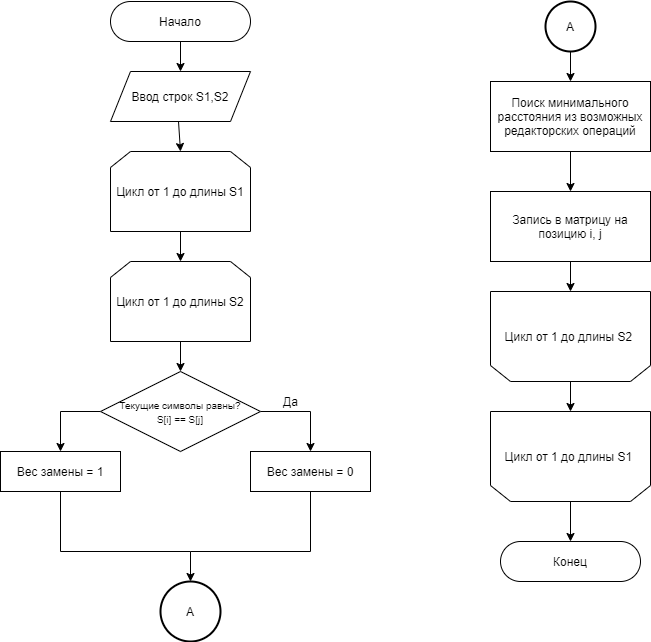
\includegraphics[width=\linewidth, height = 0.5\textheight]{iteration_leven}}
		\caption{Схема алгоритма нахождения расстояния Левенштейна. Сделана по реализации кода в приложении.\centering}
		\label{image1}
	\end{figure}

	\begin{figure}[h]
		\center{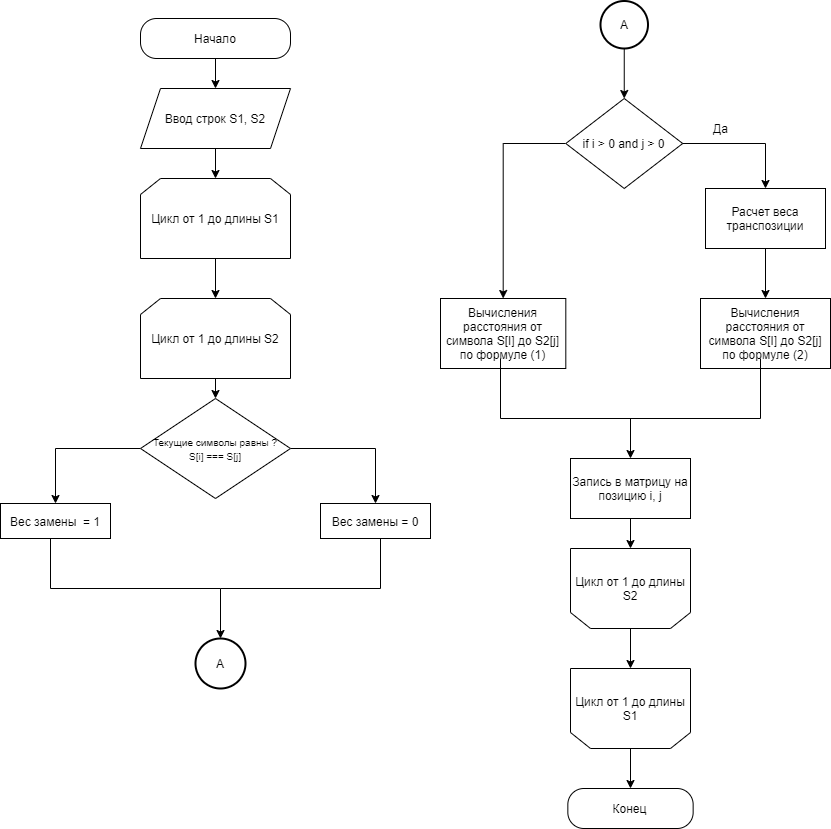
\includegraphics[width=\linewidth, height = 0.5\textheight]{damerau-leven}}
		
		\caption{Схема алгоритма нахождения расстояния Дамерау - Левенштейна. Сделана по реализации кода в приложении. \centering}
		\label{image2}
	\end{figure}

	\begin{figure}[h]
		\center{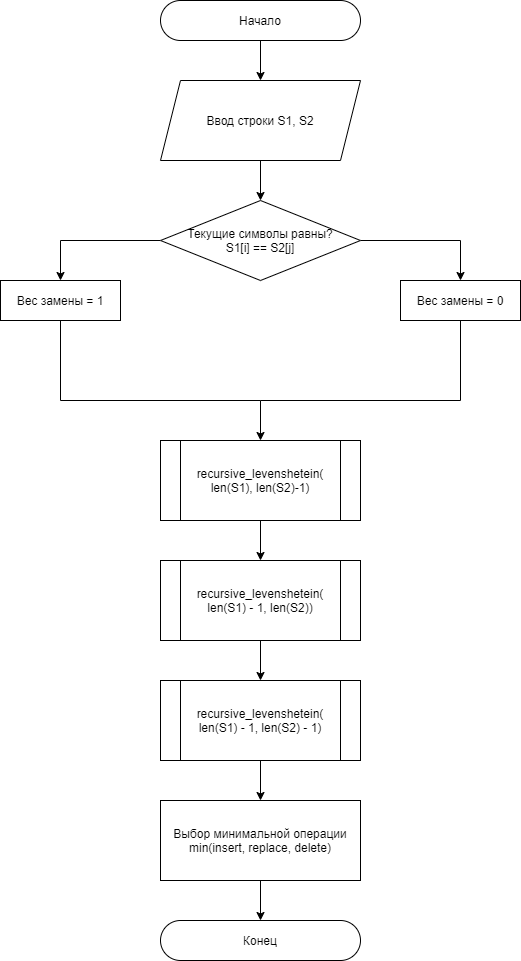
\includegraphics[width=0.5\linewidth, height = 0.7\textheight]{recursive_leven}}
		
		\caption{Схема рекурсивного алгоритма нахождения расстояния Левенштейна. Сделана по реализации кода в приложении. \centering}
		\label{image3}
	\end{figure}

	\begin{figure}[h]
	\center{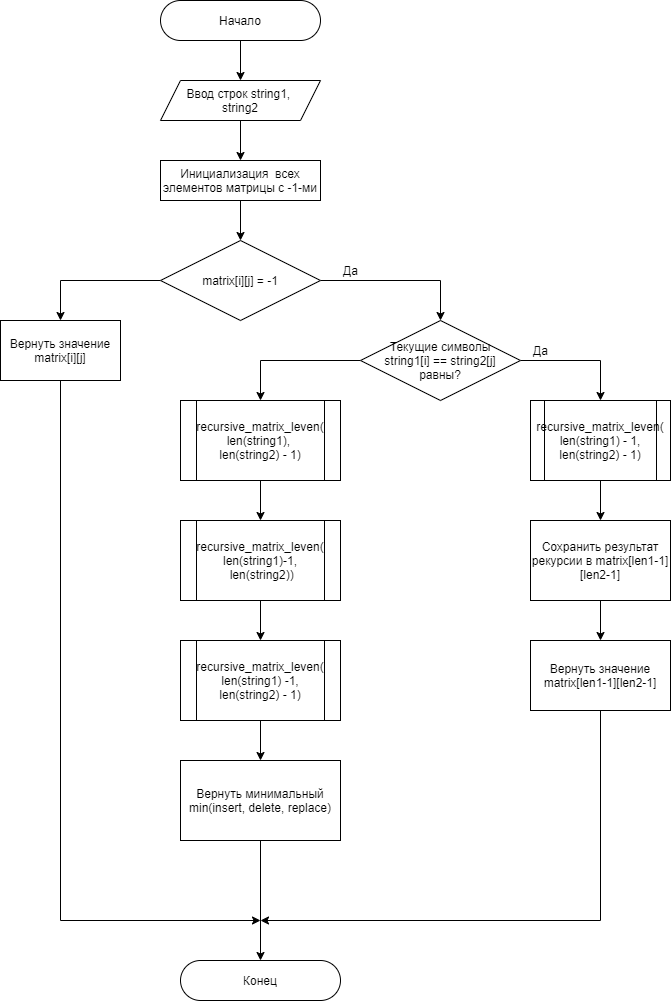
\includegraphics[ width=1\linewidth, height = 0.7\textheight]{recursive_matrix_leven}}
	
	\caption{Схема алгоритма нахождения расстояния Левенштейна с рекурсивным заполнением матрицы.Сделана по реализации кода в приложении. \centering}
	\label{image4}
\end{figure}


	

	
	\clearpage
	
	\section{Технологическая часть}
	\subsection{Выбор языка программирования}
	Python\cite{what_is_python} — это высокоуровневый язык программирования, который используется в различных сферах IT, таких как машинное обучение, разработка приложений, web, парсинг и другие.
	С ним легко работать, что сокращает время разработки. Написанный в удобочитаемом формате, Python делает процесс разработки программного обеспечения быстрым, удобным и максимально упрощенным.
	По сравнению с другими языками, Python в 5-10 раз быстрее по времени разработки, однако медленный при выполнении программ. Он обеспечивает расширенные возможности управления процессами и объектно-ориентированный дизайн, помогая как в скорости, так и в производительности.
	\clearpage

	\subsection{Методы замера времени в программе}
	\subsubsection{Время}
	Сушествует несколько способов измерения процессорного времени исполнения программы. 
	Помимо стандратного модуля $time$ есть библиотека $timeit$ \cite{timeit}. Этот модуль предоставляет простой способ найти время выполнения маленьких битов кода Python.
	$timeit$ запускает фрагмент кода миллионы раз(значение по умолчанию - 1000000), так что получаем наиболее статистически значимое измерение времени выполнения кода.
	\subsubsection{Улучшение точности замеров времени} Чтобы получить более точные результаты, каждый тест запускается несколько раз, все полученные значения времени(в тиках) суммируются и делятся на количество запусков кода. Таким образом, получаем среднее время выполнения кода.
	\clearpage
	\section{Экспериментальная часть}
	
	\subsection{Листинг кода}
	На Листингах показаны 2 - 5 показаны реализации алгоритмов для нахождения редакционного расстояния.

	\begin{lstlisting}[label=Iteration_leven,caption=Расстояние Левенштейна(итеративная реализация)]
		
	 def non_recursive_levenshtein (string1, string2):
		n1 = len(string1)
		n2 = len(string2)

		
		d = [[0  for j in range(n2+1)] for i in range(n1+1)]
		
		for i in range(n2+1):
			d[0][i] = i
		
		for i in range(n1+1):
			d[i][0] = i
		
		if n1 == 0 or n2 ==0:
			return max(n1, n2)

		for i in range(1, n1):
			for j in range(1, n2):
				d[i][j] = min(d[i-1][j] + 1, d[i][j-1] + 1, d[i-1][j-1] +is_weight(string1[i], string2[j]))

		
		for i in range(n1+1):
			for j in range(n2+1):
				print(d[i][j], end = ' ')
			print("\n")
		
	\end{lstlisting}
	\clearpage
	\begin{lstlisting}[label=recursive_leven,caption=Расстояние Левенштейна(рекурсивная реализация)]
	def recursive_leven(s1, s2):
			def recursive(n1, n2):
				if n1 == 0 or n2 == 0:
					return max(n1, n2)
		
				elif s1[n1-1] == s2[n2-1]:
					return recursive(n1-1, n2-1)
				else:
					return 1 + min(
						recursive(n1, n2 -1), #delete
						recursive(n1-1, n2), #insert
						recursive(n1-1, n2-1) # replace
					)
	return recursive(len(s1), len(s2))
	\end{lstlisting}
	\clearpage
	%Листинг3: Алгоритм для нахождения расстояния Левенштейна(с заполнением матрицы)
	\begin{lstlisting}[label=recursive_matrix,caption=Расстояние Левенштейна(рекурсивное заполнение матрицы)]
		def recursive_matrix_leven(string1, string2, matrix):
			def recursive(n1, n2):
				if n1 == 0 or n2 == 0:
					return max(n1, n2)
				for i in range(n2+1):
					matrix[0][i] = i
		
				for i in range(n1+1):
					matrix[i][0] = i
		
				if matrix[n1-1][n2-1] != -1:
					return matrix[n1-1][n2-1]
		
				if string1[n1-1] == string2[n2-1]:
					matrix[n1-1][n2-1] = recursive(n1-1, n2-1)
					return matrix[n1-1][n2-1]
				matrix[n1-1][n2-1] = 1 + min(recursive(n1, n2-1), recursive(n1-1, n2), recursive(n1-1, n2-1))
				return matrix[n1-1][n2-1]
		return recursive(len(string1),len(string2))
	\end{lstlisting}
	\clearpage
%	Листинг4: Алгоритм для нахождения расстояния Дамерау-Левенштейна(итеративная реализация).
	\begin{lstlisting}[label=damerau-leven,caption= Алгоритм для нахождения расстояния Дамерау-Левенштейна(итеративная реализация)]
		def damerau_levenshtein(string1, string2):
		n1, n2 = len(string1), len(string2)
		if n1 == 0:
			return n2
		if n2 == 0:
			return n1
		d = [[0  for j in range(n2+1)] for i in range(n1+1)]
		for i in range(n2+1):
			d[0][i] = i
		
		for i in range(n1+1):
			d[i][0] = i
		for i in range(1, n1):
			for j in range(1, n2):
				insert = d[i-1][j]+1
				delete = d[i][j-1]+1
				replace = d[i-1][j-1]+is_weight(string[i-1], string[j-1])
				minimum = min(insert, delete, replace)
				if i>1 and j >1 and
								is_weight(string[i-1], string2[j-2]) and
								is_weight(string[i-1], string2[j-1]) and
								is_weight([i-1][j-1]):
					minimum = min(minimum, d[i-2][j-2]+1)
				d[i][j] = minimum
		return d[n1][n2]
	\end{lstlisting}
	\clearpage 
	
	\subsection{Примеры работы}
	В листингах ~\ref{ex1} - ~\ref{ex4} приведены примеры работы алгоритмов.
	\begin{lstlisting}[label = ex1, caption = Пример работы алгоритмов]
		Input 1 string: aaaaa
		Input 2 string: bbb
		    b b b 
		
		  0 1 2 3 
		
		a 1 1 2 3 
		
		a 2 2 2 3 
		
		a 3 3 3 3 
		
		a 4 4 4 4 
		
		a 5 5 5 5 
		Levenshtein:  5
		Recursive Levenshtein:  5
		Damerau-Levenshtein:  5
		Recursive matrix =  5
	\end{lstlisting}
	\begin{lstlisting}[label = ex2, caption = Пример работы алгоритмов]
	Input 1 string: mama
	Input 2 string: papa
	    p a p a 
	
	  0 1 2 3 4 
	
	m 1 1 2 3 4 
	
	a 2 2 1 2 3 
	
	m 3 3 2 2 3 
	
	a 4 4 3 3 2 
	Levenshtein:  2
	Recursive Levenshtein:  2
	Damerau-Levenshtein:  2
	Recursive matrix =  2
	\end{lstlisting}
	\clearpage
	\begin{lstlisting}[label = ex3, caption = Пример работы алгоритмов]
		Input 1 string: ok
		Input 2 string: ko
		    k o 
		
		  0 1 2 
		
		o 1 1 1 
		
		k 2 1 2 
		Levenshtein:  2
		Recursive Levenshtein:  2
		Damerau-Levenshtein:  2
		Recursive matrix =  2
	\end{lstlisting}
	\begin{lstlisting}[label = ex4, caption = Пример работы алгоритмов]
		Input 1 string: cat
		Input 2 string: cat
		    c a t 
		
		  0 1 2 3 
		
		c 1 0 1 2 
		
		a 2 1 0 1 
		
		t 3 2 1 0
		Levenshtein:  0
		Recursive Levenshtein:  0
		Damerau-Levenshtein:  0
		Recursive matrix =  0
	\end{lstlisting}
	\clearpage
	
	\subsection{Показательное сравнение временных характеристик}
	Сравнение быстродействия алгоритмов Левенштейна и Дамерау-Левенштейнав матричной и рекурсивной формой в тиках приведено в таблице ~\ref{tab:vremya1}. 
	\begin{table}[h]
		\caption{\label{tab:vremya1} Временные сравнения алгоритмов.}
			\begin{center}
				\begin{tabular}{|p{70pt}|p{100pt}|p{130pt}|p{90pt}|p{70pt}|}
					\hline
					Слова & L & LR & DL & LMR\\ \hline
					5 &  6777 &18105180  & 7421 & 4715\\	\hline
					10 & 36872 &332723388 & 26163 & 5407\\ \hline
					15 & 21574 &104631506 & 25570 & 4546\\ \hline
					100 &237151 & 1045942000 & 186527 & 5570 \\ \hline
					200 &458068 & 2297609000 & 316668 & 10059 \\ \hline
					350 &1823692& 5569742500 & 664259 & 18948 \\ \hline
					500 &2064513 & 27433621866999994 & 1170698 & 29770 \\ \hline
				\end{tabular}
			\end{center}
	\end{table}\\
	Характеристики компьютера, на котором были производились замеры времени:
	\begin{enumerate}
		\item операционная система - Майкрософр Windows 10 для образовательных учреждений 10.0.18363
		\item процессор - Intel(R) Core(TM) i5-6300U CPU @2.30GHz 2.40 GHz
		\item видеокарта - Intel(R) HD Graphics 520
	\end{enumerate}
	\clearpage
	\subsection{Показательное сравнение по памяти}
	Алгоритмы Левенштйна и Дамерау-Левенштейна не отличаются друг от друга с точки зрения использования памяти. Следовательно, достаточно рассмотреть лишь разницу рекурсивной и матричной реализаций этих алгоритмов. Максимальная глубина стека вызовов при рекурсивной реализации равна сумме длин входящих строк, соответственно, максимальный расход памяти равен:
	\begin{equation}
	C(S1) + C(S2) * (2 * C(str) + 3*C(int))
	\end{equation}
	\label{pamyat1}	
	где $C$ - оператор вычисления размера, $S1, S2$ - строки, $int$ - целочисленный тип, $str$ - строковый тип.
	
	Использование памяти при итеративной реализации теорически равен:
	\begin{equation}
		C(S1+1) + C(S2+1) * C(int) + 10*C(int) + 2*C(str)
		\label{pamyat2}
	\end{equation}
	\clearpage
	\section*{Заключение} В ходе работы были сделаны следующие выводы:
	\begin{itemize}
		\item рекурсивная реализация алгоритма Левенштейна и Дамерау-Левенштейна выполняются быстрее только в случаях, когда замер одной из строк крайне мал;
		\item  итеративные реализации алгоритмов поиска расстояний Дамерау-Левенштейна и Левенштейна имеют схожую конструкцию, но алгоритм поиска расстояния Дамерау-Левенштейна из-за более сложной внутренней логики в среднем работает медленнее. 
		\item Итеративный алгоритм поиска расстояний Левенштейна и Дамерау-Левенштейна являются намного эффективнее по времени, чем их рекурсивные реализации.
	\end{itemize}
	Была достигнута цель и решены следующие задачи:
	\begin{enumerate}
		\item были рассмотрены алгоритмы поиска расстояния Левенштейна и Дамерау-Левенштейна для нахождения редакционного расстояния между строками;
		\item были реализованы данные алгоритмы на языке программирования Python;
		\item был проведен сравнительный анализ алгоритмов по затраченному времени и памяти;
		\item были приведены примеры работы всех указанных алгоритмов;
	\end{enumerate}
	\clearpage
	
	
	
	\begin{thebibliography}{4}
		\bibitem{what_is_python}	 
		Python:что нужно знать. [ЭЛ. РЕСУРС]\\
		Режим доступа: https://skillbox.ru/media/code/story\_buzunov/ \\
		(Дата обращения: 05.10.2020)
		\bibitem{timeit}
		Timeit в Python с примерами. [ЭЛ. РЕСУРС]\\
		Режим доступа: http://espressocode.top/timeit-python-examples/ \\
		(Дата обращения: 05.10.2020)
		\bibitem{levenshtein}
		Расстояние Левенштейна на Python. [ЭЛ. РЕСУРС] \\
		Режим доступа: https://tirinox.ru/levenstein-python/ \\
		(Дата обращения: 05.10.2020)\\
		\bibitem {programm_leven}
		Программная реализация алгоритма Левенштейна для устранения опечаток в записях баз данных.[ЭЛ. РЕСУРС]\\
		 Режим доступа: https://moluch.ru/archive/19/1966/ \\
		 (Дата обращения: 05.10.2020)
		 
	\end{thebibliography}

\end{document}